% !TEX root = main.tex
\documentclass[sigconf,review,anonymous]{acmart}
\usepackage{graphicx}
%% acmart loads newtxmath, which already defines \Bbbk; amssymb would clash.
\let\Bbbk\relax
\usepackage{amsmath, amssymb, amsthm}
\usepackage{stmaryrd}
\usepackage{booktabs}
\usepackage{subcaption}
\captionsetup[subfigure]{font=footnotesize, labelfont=normalfont, textfont=normalfont}

\theoremstyle{plain}
\newtheorem{lemma}{Lemma}
\newtheorem{theorem}{Theorem}
\newtheorem{assumption}{Assumption}
\newtheorem{proposition}{Proposition}
\theoremstyle{definition}
\newtheorem{definition}{Definition}
\newtheorem{corollary}{Corollary}
\theoremstyle{remark}
\newtheorem{remark}{Remark}


\newcommand{\Dd}{\mathcal{D}}
\newcommand{\Du}{\mathbb{D}}
\newcommand{\Tt}{\mathcal{T}}
\newcommand{\dataf}{\mathsf{data}}
\newcommand{\ev}[2]{\llbracket #1 \rrbracket_{#2}}
\newcommand{\bigjoin}{\mathop{\bowtie}\limits}
\newcommand{\disc}{\mathsf{disc}}
\newcommand{\reach}{\mathrm{reach}}

%% Rights / Conference Info Management
%% SIGMOD camera-ready will require specific copyright macros;
%% for submission/review, suppressing them keeps the layout clean.
\settopmatter{printacmref=false} % Suppress ACM reference block for review
\renewcommand\footnotetextcopyrightpermission[1]{} % Suppress copyright footnote for review
\pagestyle{plain} % Simple page numbering for review

%% Metadata
\title{Your Paper Title Here}

%% Author block
%% Anonymized automatically because the 'anonymous' class option is active.
\author{Anonymous Author(s)}
\affiliation{
  \institution{Institution Name}
  \city{City}
  \country{Country}
}
\email{author@domain.edu}

% Packages
\usepackage[dvipsnames,svgnames]{xcolor} % text color
\usepackage[normalem]{ulem} % wavy underlines

% Comments
\newcommand{\todo}[1]{\noindent\textcolor{red}{{\bf \{TODO}: #1{\bf \}}}}
\newcommand{\TODO}[1]{\todo{#1}}
\newcommand{\citeneeded}{\textcolor{red}{{\bf [?!]}}}
\newenvironment{draft}{\color{gray}}{\color{black}}

% Reviewers
\newcommand\rt[1]{{\color{Red}\textbf{RT}: #1}}

% Annotations
\makeatletter
\font\uwavefont=lasyb10 scaled 700
\def\spelling{\bgroup\markoverwith{\lower3.5\p@\hbox{\uwavefont\textcolor{Red}{\char58}}}\ULon}
\def\grammar{\bgroup\markoverwith{\lower3.5\p@\hbox{\uwavefont\textcolor{LimeGreen}{\char58}}}\ULon}
\def\phrasing{\bgroup\markoverwith{\lower3.5\p@\hbox{\uwavefont\textcolor{RoyalBlue}{\char58}}}\ULon}
\let\rephrase\phrasing
\newcommand\remove{\bgroup\markoverwith{\textcolor{red}{\rule[0.5ex]{2pt}{0.4pt}}}\ULon}
\newcommand\insertion{\bgroup\markoverwith{\textcolor{Green}{\rule[-0.5ex]{2pt}{0.6pt}}}\ULon}
\makeatother



\begin{document}

\begin{abstract}
Your abstract text goes here. Keep it concise, focused on the core database or data management challenge, your approach, and key experimental findings.
\end{abstract}

%% CCS Concepts and Keywords (often required for final publication)
\begin{CCSXML}

   
       10002951.10002952
       Information systems~Data management systems
       500
   
 
\end{CCSXML}

\ccsdesc[500]{Information systems~Data management systems}

\keywords{databases, query processing, distributed systems}

\maketitle

\section{Introduction}

\section{Related Work}

\section{Methodology}

\subsection{Preliminaries}

\subsection{Query Delegation in Discovery Settings}
\label{sec:authority}

Dynamically integrating conjunctive sub-queries during federated query processing 
in discovery-based querying at runtime is difficult due to the unbounded nature of
the query execution. To show this, we first introduce a sufficient
condition for correctly delegating conjunctive queries in the traditional federated case.
Then we will show how deciding whether we can correctly delegate these queries in the
discovery-based querying case is impossible when not all sources have been discovered.
 
First we define our discovery-based federated query setting in 
Definition~\ref{def:setting} and~\ref{def:reach}.

\begin{definition}[Discovery setting]
\label{def:setting}
A \emph{discovery setting} is a tuple
$W = \langle \Du, \dataf, \Dd_0, \disc \rangle$: a universe of sources $\Du$, a map
$\dataf : \Du \to 2^{\Tt}$ giving the graph each one holds, a set of seeds
$\Dd_0 \subseteq \Du$, and a \emph{discovery function} $\disc$ assigning to every BGP $B$
a map $\disc_B : \Du \times 2^{\Tt} \to 2^{\Du}$, where $\disc_B(d, \dataf(d))$ are the
sources that a retrieved $d$ exposes while $B$ is evaluated.
\end{definition}

\begin{definition}[Reachable set, reference answer]
\label{def:reach}
Iterating discovery from the seeds, let
$\Dd_{i+1} := \Dd_i \cup \bigcup_{d \in \Dd_i} \disc_B\bigl(d, \dataf(d)\bigr)$. The
\emph{reachable set} is $\reach_B(W) := \bigcup_{i \geq 0} \Dd_i$, and the
\emph{reference answer} to $B$ is $\ev{B}{G_{\reach_B(W)}}$. Correctness of a delegation
is always measured against this reference answer, never against the universe $\Du$:
sources that are never reached cannot contribute to it.
\end{definition}

\noindent

Given this definition, we recover the traditional federated query processing setting,
in which all sources are known beforehand, by taking $\Dd_0 = \Du$ 
and $\disc_B \equiv \emptyset$.

Next we define an operator to determine the \emph{relevance} of a source for a query
execution setting. Relevance records, for each triple pattern and each source, whether
that source produces matches. An example of such an operator is the usage of \textsf{ASK}
queries to determine exclusive groups in FedX~\cite{schwarte2011fedx}.

\begin{definition}[Source relevance]
\label{def:relevance}
Fix a setting $W$ and a BGP $B$, and write $\Dd := \reach_B(W)$ for its reachable set;
all that follows is relative to $\Dd$. Let $\mathcal{P}$ be the set of triple patterns.
We write $\llbracket t \rrbracket_{d}$ for the evaluation of a triple
pattern $t$ over the data of source $d$. The \emph{relevance indicator}
$\Delta : \mathcal{P} \times \Dd \to \{0,1\}$ is
\[
  \Delta(t, d) \;=\;
  \begin{cases}
    1, & \text{if } \llbracket t \rrbracket_{d} \neq \emptyset, \\[2pt]
    0, & \text{otherwise,}
  \end{cases}
\]
and $\Dd_t := \{\, d \in \Dd \mid \Delta(t,d) = 1 \,\}$ denotes the
\emph{relevant sources} of $t$.
\end{definition}

Thus, relevance means that a data source returns answers for a given triple pattern.
Next, we introduce a definition of \emph{correct} delegation of conjunctive queries to a
set of sources.

\begin{definition}[Delegation]
\label{def:delegation}
Let $B$ be a BGP, $B' \subseteq B$ the delegated fragment, and $S \subseteq \Dd$ the
(only) sources to which $B'$ is sent as a single conjunctive request, where as in
Definition~\ref{def:relevance}, $\Dd = \reach_B(W)$. Write
$G_A := \bigcup_{d \in A} \dataf(d)$ for $A \subseteq \Dd$. The delegated plan obtains for $B'$
\[
  R \;:=\; \Big( \bigcup_{d \in S} \ev{B'}{\dataf(d)} \Big)
           \;\cup\; \ev{B'}{G_{\Dd \setminus S}},
\]
and the delegation is \emph{correct} if
\[
  R \;\bowtie\; \ev{B \setminus B'}{G_{\Dd}} \;=\; \ev{B}{G_{\Dd}} .
\]
\end{definition}

This definition follows some of the definitions of federation of FedQPL~\cite{cheng2020fedqpl}.
Next we give a sufficient condition for correctly delegating conjunctive (sub)-queries to
federated sources.

\begin{theorem}[Correct delegation]
  \label{th:correct-delegation}
    Let $W$ be a \emph{federated} setting, that is $\disc_B \equiv \emptyset$, so that
    $\Dd = \reach_B(W) = \Dd_0$ is known in advance.
    Let $t_{1}, \dots, t_{n}$ be a set of triple patterns forming a BGP $B$, 
    $B' \subseteq B$ a sub-BGP, and let $d \in \Dd$. 
    For $d$ we define $\Dd^{\prime} = \Dd \setminus \{d\}$
    the set containing all other sources. 
    Then we can correctly delegate $B^{\prime}$ to $d$ if
    $\bigcup_{t_i \in B^{\prime}}
    \{\, d^{\prime} \in \Dd^{\prime} \mid \Delta(t_i, d^{\prime}) = 1 \,\} = \emptyset$
\end{theorem}
\begin{proof}
We prove the special case of Definition~\ref{def:delegation} with $S = \{d\}$, so that
$\Dd \setminus S = \Dd^{\prime}$. We assume $B^{\prime} \neq \emptyset$ and that distinct
sources use disjoint sets of blank nodes.

The argument rests on the fact that a \emph{single} triple pattern distributes over a
union of sources: for every $t$ and every $A \subseteq \Dd$,
\begin{equation}
  \ev{t}{G_{A}} \;=\; \bigcup_{e \in A} \ev{t}{\dataf(e)},
  \label{eq:distrib}
\end{equation}
since matching one pattern involves no join. Note that \eqref{eq:distrib} fails for BGPs,
which is exactly what makes delegation non-trivial.

By hypothesis no source other than $d$ is relevant to any pattern of $B^{\prime}$, so
Definition~\ref{def:relevance} gives
\begin{equation}
  \ev{t^{\prime}}{\dataf(d^{\prime})} = \emptyset
  \quad \text{for all } t^{\prime} \in B^{\prime},\ d^{\prime} \in \Dd^{\prime}.
  \label{eq:empty}
\end{equation}

\emph{Step 1.} A BGP is the join of its patterns, and each pattern distributes over the
sources by \eqref{eq:distrib}:
\[
  \ev{B}{G_{\Dd}}
  \;=\; \bigjoin_{t \in B} \ev{t}{G_{\Dd}}
  \;=\; \bigjoin_{t \in B} \ \bigcup_{e \in \Dd} \ev{t}{\dataf(e)} .
\]

\emph{Step 2.} Since $\bowtie$ is associative and commutative, the delegated fragment
splits off:
\[
  \ev{B}{G_{\Dd}} \;=\;
  \Bigl( \bigjoin_{t^{\prime} \in B^{\prime}} \bigcup_{e \in \Dd}
         \ev{t^{\prime}}{\dataf(e)} \Bigr)
  \bowtie \ev{B \setminus B^{\prime}}{G_{\Dd}} .
\]

\emph{Step 3.} As $\Dd = \Dd^{\prime} \uplus \{d\}$, the inner union splits, and by
\eqref{eq:empty} its $\Dd^{\prime}$ part is empty:
\[
  \bigcup_{e \in \Dd} \ev{t^{\prime}}{\dataf(e)}
  \;=\; \underbrace{\bigcup_{d^{\prime} \in \Dd^{\prime}}
        \ev{t^{\prime}}{\dataf(d^{\prime})}}_{=\,\emptyset}
        \;\cup\; \ev{t^{\prime}}{\dataf(d)}
  \;=\; \ev{t^{\prime}}{\dataf(d)} .
\]
Substituting into Step 2 and reassembling the join,
\begin{equation}
  \ev{B}{G_{\Dd}} \;=\;
  \ev{B^{\prime}}{\dataf(d)} \bowtie \ev{B \setminus B^{\prime}}{G_{\Dd}} .
  \label{eq:ref}
\end{equation}

\emph{Step 4.} It remains to identify $R$ from Definition~\ref{def:delegation}. Its
second term vanishes, again by \eqref{eq:distrib} and \eqref{eq:empty} and using
$B^{\prime} \neq \emptyset$:
\[
  \ev{B^{\prime}}{G_{\Dd \setminus S}}
  \;=\; \bigjoin_{t^{\prime} \in B^{\prime}} \ \bigcup_{d^{\prime} \in \Dd^{\prime}}
        \ev{t^{\prime}}{\dataf(d^{\prime})}
  \;=\; \bigjoin_{t^{\prime} \in B^{\prime}} \emptyset
  \;=\; \emptyset .
\]
With $S = \{d\}$ the first term of $R$ is the single request to $d$, so
$R = \ev{B^{\prime}}{\dataf(d)} \cup \emptyset = \ev{B^{\prime}}{\dataf(d)}$.

\emph{Conclusion.} Substituting $R$ into \eqref{eq:ref},
\[
  R \bowtie \ev{B \setminus B^{\prime}}{G_{\Dd}} \;=\; \ev{B}{G_{\Dd}},
\]
which is the correctness condition of Definition~\ref{def:delegation}.
\end{proof}

Theorem~\ref{th:correct-delegation} gives us a sufficient condition for delegating 
conjuctive sub-queries in the case where the reachable set $\Dd$ is known in advance. However, in discovery-based
querying the sources are discovered at runtime, goverened by some discovery process which returns
during the query execution. As such, determining if we can correctly delegate depends on the
\emph{state} of the discovery process, which is defined in Definition~\ref{def:discovery-state}.

\begin{definition}[Discovery state]
  \label{def:discovery-state}
  The state of a discovery setting $W = \langle \Du, \dataf, \Dd_0, \disc \rangle$ at
  time $T$ is the tuple
  \[
    W(T) \;=\; \langle \Du, \dataf, \Dd_0, \disc, \Dd(T) \rangle,
  \]
  the setting $W$ augmented with $\Dd(T)$, the set of sources that $\dataf$ has been
  called on by time $T$, subject to
  \[
    \Dd_0 \;\subseteq\; \Dd(T) \;\subseteq\; \Dd(T') \;\subseteq\; \reach_B(W)
    \qquad \text{for all } T \leq T',
  \]
  i.e.\ the seeds are discovered from the start, discovery only ever adds sources, and
  it never adds one outside what $\disc$ can reach. For any given $W(T)$ the discovery
  \emph{frontier} is
  \[
    F(T) \;=\; \Bigl( \bigcup_{d_f \in \Dd(T)} \disc\bigl(d_f, \dataf(d_f)\bigr) \Bigr)
                \setminus \Dd(T),
  \]
  the sources that are discovered but do not yet have $\dataf$ called on them.
  Discovery is complete when $F(T) = \emptyset$.
\end{definition}

Next, we introduce the concept of an observation of an engine of the discovery state 
in Definition~\ref{def:obs-equiv}, which
denotes what the engine actually can \emph{know} about its discovery setting at given time $T$.

\begin{definition}[Observationally equivalent states]
  \label{def:obs-equiv}
  A discovery state $W(T)$ records the whole world, but a query engine at time $T$ has
  access only to the \emph{observation}
  \[
    O(T) \;=\; \bigl\langle\, \Dd(T),\; \dataf|_{\Dd(T)} \,\bigr\rangle,
  \]
  the sources it has retrieved together with their contents. 
  Two states $W_1(T)$ and $W_2(T)$ are \emph{observationally equivalent}, written
  $W_1(T) \sim W_2(T)$, when $O_1(T) = O_2(T)$. Note that $F(T)$ is computable from
  $O(T)$ and $\disc$: the extent of the frontier is observable, its contents are not. A
  property of states is \emph{determined at $T$} when all states observationally
  equivalent to $W(T)$ agree on it; an engine at time $T$ can establish a property only
  if it is determined at $T$.
\end{definition}

\begin{theorem}[Correct delegation is undetermined under incomplete discovery]
  \label{th:undetermined}
  Let $W(T)$ be a discovery state for which $F(T) \neq \emptyset$. Then there exist a
  BGP $B$, a sub-BGP $B^{\prime} \subseteq B$, a set of sources
  $S \subseteq \Dd(T)$, and two states $W_1(T)$ and $W_2(T)$, both observationally
  equivalent to $W(T)$, such that $B^{\prime}$ is correctly delegated to $S$ in $W_1(T)$
  but not in $W_2(T)$. Since the engine's input is $O(T)$ and all three states share it,
  no procedure can decide whether the delegation is correct.
\end{theorem}

\begin{proof}
  We construct two states $W_1(T)$ and $W_2(T)$, both observationally equivalent to
  $W(T)$, in which $B^{\prime}$ is delegated to $S$ correctly and incorrectly
  respectively. The two agree on $\Dd_0$, $\disc$ and $\Dd(T)$, and on $\dataf$ over
  $\Dd(T)$; they differ only beyond the frontier, which is non-empty by hypothesis.

  Take $\Dd(T) = S = \{d_1\}$ and
  \[
    B^{\prime} \;=\; B \;=\; \bigl\{\, (?s, p_1, ?o_1),\ (?s, p_2, ?o_2) \,\bigr\},
  \]
  \[
    \dataf(d_1) \;=\; \bigl\{\, (s_1, p_1, o_1),\ (s_1, p_2, o_2),\ (s_2, p_1, o_3) \,\bigr\}.
  \]
  Fix some $d^{*} \in F(T)$, and let every reachable source other than $d_1$ and $d^{*}$
  hold no data. The two states are then obtained by setting
  \[
    \dataf(d^{*}) \;=\;
    \begin{cases}
      \bigl\{\, (s_3, p_2, o_4) \,\bigr\} & \text{in } W_1(T), \\[2pt]
      \bigl\{\, (s_2, p_2, o_4) \,\bigr\} & \text{in } W_2(T).
    \end{cases}
  \]
  Since $d^{*} \notin \Dd(T)$, both states induce the same observation, and so
  $W_1(T) \sim W_2(T) \sim W(T)$ holds. The reachable set differs between the two, so we
  write $G_i$ for $G_{\reach_B(W_i)}$, the union of all data reachable in $W_i(T)$. As
  only $d_1$ and $d^{*}$ hold data,
  \[
    G_1 = \dataf(d_1) \cup \bigl\{\, (s_3, p_2, o_4) \,\bigr\},
    \qquad
    G_2 = \dataf(d_1) \cup \bigl\{\, (s_2, p_2, o_4) \,\bigr\}.
  \]

  Write
  \begin{align*}
    \mu_1 &= \{?s \mapsto s_1,\ ?o_1 \mapsto o_1,\ ?o_2 \mapsto o_2\}, \\
    \mu_2 &= \{?s \mapsto s_2,\ ?o_1 \mapsto o_3,\ ?o_2 \mapsto o_4\}.
  \end{align*}
  Neither added triple matches $(?s, p_1, ?o_1)$, so
  $\ev{B^{\prime}}{\dataf(d^{*})} = \emptyset$ in both states. By
  Definition~\ref{def:delegation} we therefore have
  \[
    R_1 \;=\; R_2 \;=\; \ev{B^{\prime}}{\dataf(d_1)} \;=\; \{\mu_1\}.
  \]
  Since $B \setminus B^{\prime} = \emptyset$ we have
  $\ev{B \setminus B^{\prime}}{G_i} = \{\mu_\emptyset\}$, the join identity, so the
  correctness condition reduces to $R_i = \ev{B}{G_i}$.

  In $W_1(T)$ the added triple has subject $s_3$, which no $p_1$-triple mentions, so it
  contributes no solution and
  \[
    \ev{B}{G_1} \;=\; \{\mu_1\} \;=\; R_1 :
  \]
  the delegation is correct. In $W_2(T)$ the added triple joins with
  $(s_2, p_1, o_3) \in \dataf(d_1)$ on $?s$, so
  \[
    \ev{B}{G_2} \;=\; \{\mu_1, \mu_2\} \;\neq\; R_2 :
  \]
  the delegation is not correct.

  The triple at $d^{*}$ yields no solution on its own, and $(s_2, p_1, o_3)$ yields none
  within $d_1$; only their join does. A single conjunctive request to $d_1$ cannot produce
  it, and neither can one to $d^{*}$, so the solution is lost precisely because the join
  crosses the frontier. As $W_1(T)$ and $W_2(T)$ present the engine with the same
  observation $O(T)$ while disagreeing on correctness, no procedure reading only $O(T)$
  can decide it.
\end{proof}


\begin{lemma}[An empty frontier certifies complete discovery]
  \label{lem:frontier}
  $F(T) = \emptyset$ if and only if $\Dd(T) = \reach_B(W)$.
\end{lemma}

\begin{proof}
  $(\Rightarrow)$ The inclusion $\Dd(T) \subseteq \reach_B(W)$ holds by
  Definition~\ref{def:discovery-state}. For the converse, $F(T) = \emptyset$ says exactly
  that
  \[
    \disc\bigl(d_f, \dataf(d_f)\bigr) \subseteq \Dd(T)
    \qquad \text{for every } d_f \in \Dd(T),
  \]
  i.e.\ that $\Dd(T)$ is closed under $\disc$; and $\Dd_0 \subseteq \Dd(T)$,
  again by Definition~\ref{def:discovery-state}. By induction, if
  $\Dd_i \subseteq \Dd(T)$ then
  \[
    \Dd_{i+1} \;=\; \Dd_i \cup \bigcup_{d \in \Dd_i} \disc\bigl(d, \dataf(d)\bigr)
    \;\subseteq\; \Dd(T)
  \]
  by closure, so $\reach_B(W) = \bigcup_{i \geq 0} \Dd_i \subseteq \Dd(T)$.

  $(\Leftarrow)$ If $d \in \reach_B(W)$ then $d \in \Dd_i$ for some $i$, hence
  \[
    \disc\bigl(d, \dataf(d)\bigr) \subseteq \Dd_{i+1} \subseteq \reach_B(W).
  \]
  Thus $\reach_B(W)$ is closed under $\disc$, and $F(T) = \emptyset$ follows.
\end{proof}

\todo{Don't like the text here}
is what makes the frontier useful: $F(T) = \emptyset$ is a
condition the engine can test, whereas $\Dd(T) = \reach_B(W)$ is a statement about a
set it cannot inspect. Together with Theorem~\ref{th:undetermined} it fixes exactly when
delegation can be established at all.

\begin{corollary}[Delegation requires complete discovery]
  \label{cor:complete-discovery}
  The correctness of every delegation of a sub-BGP $B^{\prime} \subseteq B$ to a set
  $S \subseteq \Dd(T)$ is determined at $T$ if and only if $F(T) = \emptyset$.
\end{corollary}

\begin{proof}
  $(\Leftarrow)$ Let $F(T) = \emptyset$ and let $W_1(T), W_2(T)$ be observationally
  equivalent to $W(T)$. As $F(T)$ is computable from $O(T)$, both have an empty frontier,
  so $\Dd = \reach_B(W) = \Dd(T)$ in both by Lemma~\ref{lem:frontier}. Then
  $G_{\Dd} = \bigcup_{e \in \Dd(T)} \dataf(e)$ agrees in both, and since
  $S \subseteq \Dd(T) = \Dd$, so do $G_{\Dd \setminus S}$ and $\dataf(d)$ at each
  $d \in S$. Every term of the condition of Definition~\ref{def:delegation} therefore
  agrees, and with it the verdict.

  $(\Rightarrow)$ By contraposition. If $F(T) \neq \emptyset$, then
  Theorem~\ref{th:undetermined} supplies a $B^{\prime}$, an $S$, and two states
  observationally equivalent to $W(T)$ that disagree on the correctness of delegating
  $B^{\prime}$ to $S$. That delegation is not determined at $T$.
\end{proof}

\subsection{Authority Claims}

From Corollary~\ref{cor:complete-discovery}, runtime federation in discovery-based
querying is impossible until every source is discovered. With source counts in the
thousands~\todo{cite here}, this is infeasible.

However, while classical query semantics require all data to be considered in query execution,
this is not always an intuitive requirement. 
Consider a federation of product catalogues, in which a manufacturer publishes the
specifications of the products it makes while resellers and comparison services
republish copies of them. A query over a product's specification is answered from the
manufacturer alone. However, if any copies of, different, or wrong specifications exist 
in the federation, they are considered equally `true'.


We will work towards a query execution model that resolves this observation while
also allowing the delegation of queries \emph{during} query execution.
First we introduce the concept of a \emph{composite source},
an aggregating view over sources in $\Du$ which contains no data of its own.

\begin{definition}[Composite source]
\label{def:composite}
  Fix a setting \\ $W = \langle \Du, \dataf, \Dd_0, \disc \rangle$. A source $c \in \Du$ is
  \emph{composite} when it holds no data of its own and is instead given by a set
  $\Dd_c \subseteq \Du$ of sources it aggregates. It contains all of their data,
  \[
    \dataf(c) \;=\; \bigcup_{d \in \Dd_c} \dataf(d),
  \]
  and a request to $c$ is evaluated over all of it. Sources that are not composite are
  \emph{base} sources. We require the aggregation relation to be well-founded 
  such that no source aggregates itself either directly or through a chain. 
  Thus, when unfolding $\dataf(c)$ it is expressed
  in base sources.
\end{definition}

In the case $\Dd_c = \{d\}$ with $d$ a base source, $\dataf(c) = \dataf(d)$. Then,
$c$ is equivalent to $d$.

\todo{Add this to after claim is defined} 
and interchangeable when $c$ claims (Def.~\ref{def:claim}) nothing. 

% as far as its data goes, $c$ \emph{is} $d$. A degenerate composite that claims nothing
% (Definition~\ref{def:claim}) is interchangeable with $d$ under every definition below, so
% in proofs we may treat a base source as a degenerate composite that claims nothing, and a
% single document that does claim as a degenerate composite that does.


Next we introduce \emph{claims}, which declare a subset of data the composite source
aggregates over that matches a certain criterion. 

\begin{definition}[Claim]
\label{def:claim}
A composite source $c$ may \emph{declare} a claim. A claim is a \emph{triple-wise}
criterion $\sigma_c : \Tt \to \{0, 1\}$, an indicator function mapping triples to 
claim membership.

% i.e.\ $\sigma_c(G) = \{\, t \in G \mid \sigma_c(\{t\}) = \{t\} \,\}$, and $c$
% \emph{claims} $\tau$ when $\sigma_c(\{\tau\}) = \{\tau\}$: the triples $\sigma_c$ selects
% are to be taken from $c$ and from no other source. Write $\mathcal{C} \subseteq \Du$ for
% the composite sources that declare.
\end{definition}


A claim is published with $c$ and thus observed once $c$ is retrieved. 
The core idea on which our query execution model builds is the \emph{principle of
exclusive claims}: queries are answered as if every claim were exclusive, that is, as if
no source other than $c$ held a triple claimed by $c$.
Like the closed-world assumption, this does not state how the federation environment
is; it fixes how we answer queries over it. The data need not satisfy it, and on the Web
it often does not. Definition~\ref{def:claim-semantics} makes the principle precise by
fixing the answer on any data, and the engine enforces that answer, which we discuss in
Section~\todo{?}

% Where the data violate it, we answer over the largest part of
% the data that satisfies it:
% \[
%   G^{\alpha}_A \;=\; \bigcup_{d \in A}
%   \bigl\{\, t \in \dataf(d) \;\bigm|\; d \text{ claims } t
%   \ \text{ or no } c \in \Dd \text{ claims } t \,\bigr\}.
% \]

% \begin{proposition}
% Under Assumption~\ref{as:disjoint}, $G^{\alpha}_{\Dd}$ is obtained by removing from each
% source exactly the triples Assumption~\ref{as:exclusive} forbids it to hold, and no
% others.
% \end{proposition}

Claims indicate that a composite source is the only source for answers for triples that matched
the claim indicator function. Engines can then reason about this claim to determine
for what data delegating BGPs to composite sources declaring a claim is correct.
As an example, in the product catalogue federation,
the manufacturer declares that statements about its products are to be taken from it
alone, so that copies held by resellers are disregarded.

Nothing so far prevents a source from claiming data it should not be allowed to. 
On the Web, any source could claim authority over, for example, DBpedia without being
affiliated with it, and thereby drop every DBpedia result held elsewhere. We
therefore bound each claim by what its source is entitled to.

\begin{definition}[Admissibility, effective claim]
\label{def:admissible}
An \emph{admissibility function} assigns every composite $c$ a criterion
$\rho_c : \Tt \to \{0,1\}$, the triples $c$ is entitled to claim. It is part of the
setting, not of any declaration, and depends only on the triple and the identity of $c$.
The \emph{effective claim} of $c$ is
\[
  \alpha_c(t) \;=\; \sigma_c(t) \cdot \rho_c(t),
\]
with $\alpha_d \equiv 0$ for base sources and for composites that declare nothing. A
source $d$ \emph{claims} $t$ when $\alpha_d(t) = 1$, and the principle of exclusive claims
is read with effective claims.
\end{definition}

An illegitimate claim thus shrinks to its admissible part rather than being rejected
whole: a composite claiming both DBpedia and its own namespace keeps the latter.

\begin{definition}[Claim semantics]
\label{def:claim-semantics}
A triple $t \in \dataf(d)$ is \emph{admitted from} $d$ if
\begin{equation}
  \label{eq:admitted}
  \alpha_d(t) = 1 \quad\text{or}\quad \alpha_c(t) = 0 \text{ for all } c \in \Dd \setminus \{d\},
\end{equation}
and for $A \subseteq \Dd$ the \emph{claim-respecting graph} is
\[
  G^{\alpha}_A \;=\; \bigcup_{d \in A}
  \{\, t \in \dataf(d) \mid t \text{ is admitted from } d \,\}.
\]
The
\emph{claim semantics} of $B$ is $\ev{B}{G^{\alpha}_{\Dd}}$. It replaces the reference
answer of Definition~\ref{def:reach}, and correctness of a delegation
(Definition~\ref{def:delegation}) is measured with $G^{\alpha}_A$ in place of $G_A$.
\end{definition}

Thus, any claimed triple only occurs within the source that claims it, while unclaimed
triples are left in the data as-is. If no source claims
anything, $G^{\alpha}_A = G_A$ and the claim semantics is the reference answer of
Definition~\ref{def:reach}.

\todo{Possibly tie to literature here about subwebs and relational?}

We keep admissibility abstract until Section~\ref{sec:namespace-claims}, where we
instantiate it by namespaces; the results in between hold for any admissibility function.

\begin{assumption}[Disjoint claims]
\label{as:disjoint}
No triple is claimed by two sources: for $c \neq c'$ and every $t \in \Tt$,
$\alpha_c(t) \cdot \alpha_{c'}(t) = 0$.
\end{assumption}

Section~\ref{sec:namespace-claims} gives a sufficient condition for namespace claims. We
discuss relaxing the assumption in Section~\ref{sec:overlap}.~\todo{What happens if we
relax this?}



% \emph{Authority} is the question of \emph{who may speak} about a term. Following the
% Linked Data principles, the document obtained by dereferencing an IRI is the
% distinguished source of statements about that IRI. \citet{hogan2009authoritative}
% made this operational to prevent \emph{ontology hijacking}, and
% \citet{harth2012completeness} generalised it into a lattice of \emph{authority types}
% that record whether a triple was retrieved from the document of its subject, its
% predicate, or its object. Authority is a \emph{filter}: it discards data, and it is
% chosen by the consumer.

% \emph{Completeness} is the question of \emph{what is guaranteed to be present}. In the
% relational setting this is Motro's split of a source into an available and an ideal
% instance~\cite{motro1989integrity}, and Levy's local completeness
% statements~\cite{levy1996complete,razniewski2011completeness};
% \citet{darari2013completeness,darari2018management} transported it to RDF as
% statements $\mathrm{Compl}(P_1 \mid P_2)$ asserting that a source holds every ideal
% answer to $P_1$ under condition $P_2$. Completeness is an \emph{obligation}: it adds
% nothing to the data, and it is undertaken by the publisher.

% Neither ingredient alone licenses what we need. Authority alone does not let us skip a
% source; completeness alone does not let us disregard the statements other sources make
% about the same subjects. Their conjunction does, and we make that conjunction the one
% assumption on which the rest of the paper rests.

% \subsubsection{Data model}

% We use the standard model of a Web of Linked Data~\cite{hartig2012foundations},
% refined with partial documents as in~\cite{bogaerts2021subweb}. Let $\mathcal{U}$,
% $\mathcal{B}$ and $\mathcal{L}$ be the pairwise disjoint sets of IRIs, blank nodes and
% literals, and $\Tt = (\mathcal{U} \cup \mathcal{B}) \times \mathcal{U} \times
% (\mathcal{U} \cup \mathcal{B} \cup \mathcal{L})$ the set of triples. A \emph{Web of
% Linked Data} (WoLD) is a tuple $W = \langle D, \mathsf{data}, \mathsf{adoc} \rangle$
% with $D$ a countable set of documents, $\mathsf{data} : D \to 2^{\Tt}$ mapping
% each document to a finite graph, and $\mathsf{adoc} : \mathcal{U} \rightharpoonup D$
% the partial dereferencing function. We write $\mathsf{AllData}(W) = \bigcup_{d \in D}
% \mathsf{data}(d)$, and $G|_S = \{ (s,p,o) \in G \mid s \in S \}$ for the restriction
% of a graph to subjects drawn from $S \subseteq \mathcal{U}$.

\subsection{Delegating Conjunctive Queries}
Under this query execution model, we now show that correct delegation to composite
sources can be established under \emph{incomplete} discovery.

\begin{lemma}[Claimed triples occur only in their claimant]
\label{lem:exclusive}
Under Assumption~\ref{as:disjoint}, let $c \in \Dd$ claim $\tau$. Then $\tau$ is
admitted from no source $d \neq c$. Consequently, for every $A \subseteq \Dd$,
$\tau \in G^{\alpha}_A$ implies $c \in A$ and $\tau \in \dataf(c)$.
\end{lemma}

\begin{proof}
Suppose $\tau$ is admitted from some $d \neq c$. The second clause of
\eqref{eq:admitted} fails, as $c \in \Dd \setminus \{d\}$ claims $\tau$. So the first
holds and $d$ claims $\tau$, contradicting Assumption~\ref{as:disjoint}.
\end{proof}

A delegated composite answers over all of $\dataf(c)$, so its answer must be filtered
to what the claim semantics admits. The engine can always check the claim of $c$, as
$\alpha_c$ is known once $c$ is retrieved. For a BGP $B'$ we therefore keep the solutions
whose matched triples $c$ all claims,
\[
  \Phi_c(\Omega) \;=\; \bigl\{\, \mu \in \Omega \;\bigm|\; c \text{ claims } \mu(t)
  \text{ for every } t \in B' \,\bigr\},
\]
and evaluate the rest of $B'$ over the other sources. This refines
Definition~\ref{def:delegation} for $S = \{c\}$:
\[
  R \;:=\; \Phi_c\bigl(\ev{B'}{\dataf(c)}\bigr) \;\cup\;
  \ev{B'}{G^{\alpha}_{\Dd \setminus \{c\}}}.
\]
Unclaimed triples held by $c$ are also held by the sources it aggregates, so they are
found by the second term, provided these sources are reachable.

\begin{assumption}[Reachable aggregation]
\label{as:agg-reach}
If a composite $c$ is in $\Dd$, so is every source it aggregates: $\Dd_c \subseteq \Dd$.
\end{assumption}

This holds, for instance, when a composite exposes its sources and $\disc$ follows them.
What can go wrong is a solution that the two terms split between them.

\begin{definition}[Claim-uniform sub-query]
\label{def:uniform}
Let $G = G^{\alpha}_{\Dd}$. A BGP $B'$ is \emph{claim-uniform} for a composite $c$ if
every $\mu \in \ev{B'}{G}$ has $c$ claim either all of $\mu(t)$, $t \in B'$, or none of
them.
\end{definition}

\begin{theorem}[Delegation to a claim]
\label{th:claim-delegation}
Under Assumptions~\ref{as:disjoint} and~\ref{as:agg-reach}, let $B' \subseteq B$ be
non-empty, $c \in \Dd(T)$ a composite, and $G = G^{\alpha}_{\Dd}$. Then
$R = \ev{B'}{G}$ if and only if $B'$ is claim-uniform for $c$; in that case delegating
$B'$ to $c$ is correct. Consequently, whenever claim uniformity follows from $B'$ and
$\alpha_c$ alone, correctness is determined at $T$, whether or not $F(T) = \emptyset$.
\end{theorem}

\begin{proof}
Write $G_c := G^{\alpha}_{\{c\}}$ and $G_{\neg c} := G^{\alpha}_{\Dd \setminus \{c\}}$.

($R \subseteq \ev{B'}{G}$.) A triple of $\dataf(c)$ that $c$ claims is admitted from
$c$ by the first clause of \eqref{eq:admitted}, so a solution kept by $\Phi_c$ maps into
$G_c \subseteq G$. The second term maps into $G_{\neg c} \subseteq G$.

($\ev{B'}{G} \subseteq R$ under uniformity.) Let $\mu \in \ev{B'}{G}$. If $c$ claims every
$\mu(t)$, each is admitted only from $c$ by Lemma~\ref{lem:exclusive}, hence lies in
$\dataf(c)$; so $\mu \in \ev{B'}{\dataf(c)}$ and $\Phi_c$ keeps it. If $c$ claims no
$\mu(t)$, let $\tau = \mu(t)$ be admitted from $d$. If $d \neq c$, then
$\tau \in G_{\neg c}$. If $d = c$, then $\tau$ is unclaimed, as $c$ does not claim it and
by \eqref{eq:admitted} no other source does; it is held by some $d' \in \Dd_c$, which lies
in $\Dd$ by Assumption~\ref{as:agg-reach} and admits $\tau$, so again
$\tau \in G_{\neg c}$. Hence $\mu \in \ev{B'}{G_{\neg c}}$.

(Necessity.) Let $\mu \in \ev{B'}{G}$ mix claimed and unclaimed triples, with $c$
claiming $\mu(t_1)$ but not $\mu(t_2)$. Then $\Phi_c$ discards $\mu$, and
$\mu(t_1) \notin G_{\neg c}$ by Lemma~\ref{lem:exclusive}, so $\mu \notin R$.

Given $R = \ev{B'}{G}$, $R \bowtie \ev{B \setminus B'}{G} = \ev{B}{G}$, which is
correctness. Finally, $\Phi_c$ depends only on $\alpha_c$, and the argument quantifies over
every source of $\Dd$, discovered or not; so whenever uniformity is guaranteed by $B'$ and
$\alpha_c$ alone, the verdict is the same in every state observationally equivalent to
$W(T)$.
\end{proof}

Theorem~\ref{th:claim-delegation} pins down what remains of the adversary of
Theorem~\ref{th:undetermined}: it wins only by building a solution that mixes a triple
claimed by $c$ with one that is not, so that the join crosses the boundary of $c$. Claim
uniformity is exactly the absence of such solutions. A triple placed behind the frontier
that $c$ claims is admitted only from $c$, and one that $c$ does not claim is found by the
second term; neither breaks a uniform sub-query.

The simplest uniform case needs no knowledge of the data at all: if $c$ claims every
triple matching every pattern of $B'$, all solutions are fully claimed. We say $B'$ is
then \emph{within the claim} of $c$; the second term of $R$ is empty and
$\Phi_c$ is the identity. Under namespace claims (Section~\ref{sec:namespace-claims}) this
requires constant subjects in the namespace of $c$. Uniformity is much weaker: it only
forbids mixed solutions, and Section~\ref{sec:shapes} shows that subject-determined
claims guarantee it for star-shaped sub-queries regardless of the data. A composite that
claims nothing has $\Phi_c(\Omega) = \emptyset$, so delegating to it is vacuous: we
delegate only to claimants, and a single document only as a degenerate composite that
declares a claim.


\todo{Lemma on how theorem 1 holds if we filter any sources in scope 
of $c$ both backwards and forwards in time. Mention how the filtering changes
nothing given the assumptions / semantics of our model}
\begin{proof}
  Sketch
  Part 1. If we filter -> Theorem~\ref{th:correct-delegation} can be directly applied
  Part 2. Filtering is possible: forward -> easy just take $\disc()$ 
  and apply setminus of in scope documents.
  Backwards -> deduplication, we only have duplicate results. So filter any
  intermediate results at time T in data(scope) and filter any produced results
  in composite resource on B prime
\end{proof}


\subsection{Monotonicity}
\label{sec:monotonicity}

In classical discovery-based querying, a result is sound the moment it is produced: as
$\Dd(T)$ grows, so does $G_{\Dd(T)}$, and BGP evaluation is monotone. Claims break this,
as discovering a composite can disregard triples that were already used. We make this
precise for the answer an engine can compute at time $T$, which can only take the claims
of retrieved composites into account.

\begin{definition}[Answer at time $T$]
\label{def:answer-at-T}
For a discovery state $W(T)$, with claims under $\alpha$, let
\[
  G^{T} \;=\; \bigcup_{d \in \Dd(T)}
  \bigl\{\, t \in \dataf(d) \;\bigm|\; d \text{ claims } t
  \ \text{ or no } c \in \Dd(T) \text{ claims } t \,\bigr\},
\]
and $\Omega(T) = \ev{B}{G^{T}}$. The answer is \emph{monotone} if
$\Omega(T) \subseteq \Omega(T')$ whenever $T \leq T'$.
\end{definition}

Once discovery is complete, $\Dd(T) = \Dd$ by Lemma~\ref{lem:frontier} and
$G^{T} = G^{\alpha}_{\Dd}$, so $\Omega(T)$ is the answer under claims. Without claims,
$G^{T} = G_{\Dd(T)}$ and $\Omega$ is monotone.

\begin{proposition}[Claims break monotonicity]
\label{prop:non-monotone}
There is a setting with times $T \leq T'$ such that $\Omega(T) \not\subseteq \Omega(T')$.
\end{proposition}

\begin{proof}
Take $B = \{(?s, p, ?o)\}$ and a composite $c$ that claims $\tau = (s, p, o)$. Let a
base source $d \notin \Dd_c$ hold $\tau$ while $\tau \notin \dataf(c)$, and let $d$ be
retrieved before $c$. If $\Dd(T) = \{d\}$, then
$\mu = \{?s \mapsto s,\ ?o \mapsto o\} \in \Omega(T)$. Once $c \in \Dd(T')$, $c$ claims
$\tau$, so $\tau$ is no longer admitted from $d$, nor from $c$ as $\tau \notin \dataf(c)$.
Hence $\mu \notin \Omega(T')$.
\end{proof}

The triple $\tau$ is claimed by $c$ but held only elsewhere; under namespace claims it is
a statement by $d$ about a resource in the namespace of $c$. It is exactly the kind of
triple the adversary of Theorem~\ref{th:undetermined} places behind
the frontier, and exactly what Theorem~\ref{th:claim-delegation} needs disregarded.
Non-monotonicity is thus the price of delegation under incomplete discovery rather than
an artefact of our definitions.~\todo{Formalise as a necessity result?} It is, however,
confined to such triples.

\begin{definition}[Covered triple]
\label{def:covered}
A triple $t$ is \emph{covered} if every composite $c \in \Dd$ that claims $t$ also holds
it, $t \in \dataf(c)$.
\end{definition}

\begin{lemma}[Covered solutions are stable]
\label{lem:covered-stable}
Under Assumption~\ref{as:disjoint}, let $\mu \in \Omega(T)$ be such that $\mu(t)$ is
covered for every $t \in B$. Then $\mu \in \Omega(T')$ for every $T' \geq T$, and
$\mu \in \ev{B}{G^{\alpha}_{\Dd}}$.
\end{lemma}

\begin{proof}
Let $t \in B$ and $\tau = \mu(t) \in G^{T}$, so some $d \in \Dd(T)$ holds $\tau$. By
Assumption~\ref{as:disjoint} at most one source claims $\tau$. If no source of
$\Dd(T')$ claims it, $\tau$ is admitted at $T'$ from $d \in \Dd(T')$. Otherwise its
claimant $c \in \Dd(T')$ holds $\tau$, as $\tau$ is covered, and $\tau$ is admitted from
$c$. Hence $\mu(B) \subseteq G^{T'}$, and $\mu \in \Omega(T')$ as
$\mathrm{dom}(\mu) = \mathrm{var}(B)$. The same argument with $\Dd$ in place of
$\Dd(T')$ gives $\mu \in \ev{B}{G^{\alpha}_{\Dd}}$.
\end{proof}

Which triples are covered depends on admissibility. For namespace claims it follows from
where a triple is stored, which Section~\ref{sec:namespace-claims} uses to resolve claim
status in practice.

\subsection{Subject-Namespace Claims}
\label{sec:namespace-claims}

The results so far hold for any admissibility function satisfying
Assumption~\ref{as:disjoint}. Two further questions need more structure: when a
sub-query whose patterns have variable subjects can be delegated, and how an engine
settles claim status in practice. Both rely on claims that are decided by the subject of
a triple alone.

\begin{definition}[Subject-determined claims]
\label{def:subject-determined}
Claims are \emph{subject-determined} if for every composite $c$ there is a set of terms
$S_c$ such that $\alpha_c(t) = 1$ iff $\mathrm{subj}(t) \in S_c$.
\end{definition}

For this work we instantiate admissibility by namespaces, as discovery-based querying on
the Web identifies sources by IRI. With $\mathrm{ns}(c)$ the namespace of the IRI of $c$,
\[
  \rho_c(t) = 1 \iff \mathrm{subj}(t) \in \mathrm{ns}(c),
\]
and a composite that declares claims its whole namespace, $\sigma_c = \rho_c$. Claims are
then subject-determined with $S_c = \mathrm{ns}(c)$. A composite with namespace
\url{http://example.org/} thus claims every triple whose subject starts with it.
$\rho_c$ depends only on the identity of $c$, so the engine knows it as soon as it
discovers $c$, whatever lies behind the frontier. Admissibility bounds what $c$ may
\emph{claim}, not what it may \emph{aggregate}; for the latter, write
$\mathrm{iri}(d)$ for the IRI of a source $d$.

\begin{assumption}[Namespace aggregation]
\label{as:ns-aggregation}
A composite aggregates every source in its namespace: if
$\mathrm{iri}(d) \in \mathrm{ns}(c)$ then $d \in \Dd_c$.~\todo{align with subweb paper}
\end{assumption}

The picture is that of horizontal partitioning, with each composite the sole source of
record for a region of the subject space. The difference is that the partitioning is
declared by the participants rather than imposed by a coordinator, so no global catalogue
of it exists and both the participants and the partitioning are discovered during
execution. Assumption~\ref{as:disjoint} holds when no composite's namespace extends
another's. Disjoint aggregation alone does not suffice: a composite on
\url{http://example.org/} and one on \url{http://example.org/a/} may aggregate disjoint
documents and still both claim a triple about \url{http://example.org/a/x}.

\subsubsection{Resolving claim status}
\label{sec:claim-status}

Call $t \in \dataf(d)$ \emph{local} if no composite namespace separates its subject from
its source: for every composite $c$, $\mathrm{subj}(t) \in \mathrm{ns}(c)$ implies
$\mathrm{iri}(d) \in \mathrm{ns}(c)$. Under Assumption~\ref{as:ns-aggregation} a local
triple is covered, since a composite claiming it has $\mathrm{subj}(t) \in \mathrm{ns}(c)$,
hence $d \in \Dd_c$ and $t \in \dataf(c)$. By Lemma~\ref{lem:covered-stable}, solutions
built from local triples are sound as soon as they are produced; only solutions using a
non-local triple, a statement about a resource in another namespace, can be invalidated
by later discovery.

\begin{remark}[Resolving claim status by request]
\label{rem:claim-lookup}
In practice the engine need not wait for discovery to settle whether a non-local triple
$t$ is claimed. By Assumption~\ref{as:disjoint} at most one composite can claim $t$, and
under namespace admissibility its location is fixed by $\mathrm{subj}(t)$ alone: it is the
composite, if any, whose namespace contains $\mathrm{subj}(t)$. The engine can therefore
resolve the claim status of $t$ with a request to this possible aggregator, for example
by looking up an advertised composite along the path of $\mathrm{subj}(t)$ and, if one
claims $t$, asking it whether it holds $t$. Including these lookups in $\disc$ makes the
aggregator part of $\reach_B(W)$, so the outcome agrees with the answer under claims. An
engine that resolves the status of every non-local triple before using it emits only
solutions that remain valid, at the cost of one lookup per foreign namespace and one
membership check per non-local triple, rather than a wait for the frontier to empty.
This mirrors authoritative reasoning, where authority is decided per term by
dereferencing~\cite{hogan2009authoritative}.~\todo{Mechanism for advertising a
composite, and for establishing that none exists: storage description, link header?}
\end{remark}

\subsubsection{Star- and chain-shaped sub-queries}
\label{sec:shapes}

Subject-determined claims make the claim status of a matched triple a function of the
binding of its subject. For a star whose patterns share the subject variable $?s$, all
triples matched by a solution $\mu$ have subject $\mu(?s)$, so either $c$ claims all of
them or none. The star is therefore claim-uniform for every composite, whatever the data,
and Theorem~\ref{th:claim-delegation} applies at any time $T$; $\Phi_c$ keeps the
solutions with $\mu(?s) \in S_c$. Patterns with distinct subject variables, as in chains,
admit mixed solutions.~\todo{Formalise for stars and size-2
chains}

\todo{Section indicating how anchor variables are required to correctly filter out partial results}
\todo{This then makes stars and size 2 chains attractive candidates to reduce client work, while
longer chains can't really be pruned.}

\subsection{Adaptive Query Planning with Composite Sources}
Given the capability of delegating these sub queries, we must now move to the system-side of
our problem. Specifically, due to the dynamic discovery of composite sources and the uncertainty
of capabilities of these sources, using a static query plan is difficult.

\todo{Text referencing Figure~\ref{fig:integration}}

\begin{figure}[t]
  \centering
  \begin{subfigure}[b]{0.37\columnwidth}
    \centering
    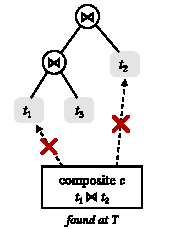
\includegraphics{figures/static-plan.pdf}
    \caption{Static plan: $t_1$ and $t_2$ lie in different subtrees, so $c$ cannot be
      added to the plan.}
    \label{fig:static-plan}
  \end{subfigure}\hfill
  \begin{subfigure}[b]{0.6\columnwidth}
    \centering
    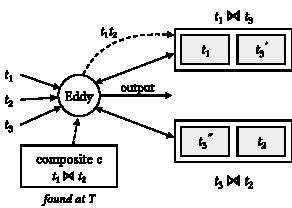
\includegraphics{figures/eddy-join-state.pdf}
    \caption{Eddy: routing history split $t_3$ into $t_3'$ and $t_3''$ across the joins,
      so the $t_1 t_2$ tuples of $c$ probe only $t_3'$.}
    \label{fig:eddy-join-state}
  \end{subfigure}
  \caption{\todo{caption}}
  \label{fig:integration}
\end{figure}

\todo{Show that even if we use many alternative plans we can still run into issues with overlapping
composite sources}

\todo{Stems!}
\label{sec:planning}

\subsection{Correctness}

\subsubsection{Overlapping Sources}
\label{sec:overlap}
Correctness when doing overlapping sources is difficult blabla, cases: Overlapping domain,
overlapping triple patterns, both, neither.
Given the time dimension, how do we decide what is possible

\subsection{Discovery}

\section{System Application}
To evaluate the performance impact of delegating sub-queries we implement 
hybrid federated link traversal-based query processing. Specifically, within solid blabla

Note this is a concrete application of the stuff introduced here, which is not limited to Solid
and link traversal.


\section{Evaluation}
TODO: Ensure correctness of multiple composite resources!!
Experiments: 
- Full benchmark and abalations
- Client-scaling test (find server-side usage and client-side scaling behavior)
- Test query with increasing pod depth to find answer
- Query where linear is fastest to delegate with single pod 
(show star-only fails and cost-based fails)
- Query where linear is fastest to delegate with multiple pods (show if cost-based doesn't fail)
- Query where star is fastest multiple pods (show if cost-based doesn't fail)
- Multiple vs Single pod query

\section{Conclusion}
Summarize results and point to future work.

%% Bibliography
\bibliographystyle{ACM-Reference-Format}
\bibliography{references/references}


%% ---------------------------------------------------------------
%% Superseded draft of the authoritativeness subsection, kept for reference.
%% ---------------------------------------------------------------
% \subsection{Authoritativeness}
% This is a working draft copy output. This needs to be better aligned with literature
% on authoritativeness and with justification. This will be the core assumption we build our theory on:
% 
% 
% Let Pod $A$ expose a composite resource $CR$ whose query is the path
% \[
% tp_1 = {?s}\ \langle p_1\rangle\ {?o_1}, \qquad
% tp_2 = {?o_1}\ \langle p_2\rangle\ {?o_2}.
% \]
% 
% A composite resource does not answer for the whole web, nor necessarily for the whole
% pod that publishes it. What it answers for is a parameter of the resource, and the entire
% development below is relative to it.
% 
% \begin{definition}[Authority scope]
% A composite resource $CR$ declares an \emph{authority scope} $S$, a set of RDF terms. We
% write $t \in CR$ for $t \in S$.
% \end{definition}
% 
% \begin{assumption}[Scope completeness]
% \label{as:scope}
% Every triple whose subject lies in $S$ belongs to the dataset over which $CR$ evaluates
% its query.
% \end{assumption}
% 
% Paste two: 
% \textbf{The ``Authoritative'' Assumption}
% We posit that a given source, with possible sub-sources in a decentralized environment is the authoritative source \textit{only} for subjects that share that source's base URL.
% Let $P$ be a source with a base URL $U_P$. Let $R_D$ be a derived resource obtained from $P$.
% The constraint for authoritative data is defined as:
% \begin{equation}
%     \forall t \in R_D, \quad \text{Authoritative}(t) \iff \text{subject}(t) \text{ startsWith } U_P
% \end{equation}
% 
% In the context of Solid, an example decentralized environment this assumption is logical. If a pod represents a person, then accepting statements about this person only in their own pod is common sense. My pod could claim to be friends with the Pope, however if the Pope does not also make this statement it is probably false.
% Future work could investigate the use of authoritativeness claims, where one data source indicates which other sources are authoritative, however this would again complicate establishing exclusive groups and would require standardization efforts.
% 
% 
% Delegating conjunctive sub-queries with more than one triple pattern requires

\end{document}